\documentclass[10pt,a4paper,final]{article}

\usepackage[latin1]{inputenc}
\usepackage{amsmath}
\usepackage{amsfonts}
\usepackage{amssymb}
\usepackage{graphicx}

\begin{document}

\section{General}

Assuming that we have some data split into training, (validation), and test data, using the training data, we can construct the probabilities for the following ideas for each person class. The training data might be picked randomly across time for each person to have better probability distribution depending on which idea we use.

\textbf{Assumption:} The number of persons are known and fixed. At the moment, new persons will be forcefully classified into one of the person class.

\section{First Idea}

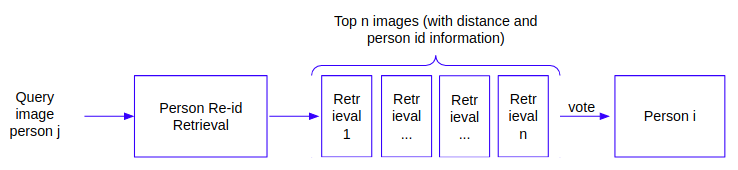
\includegraphics[width=\textwidth]{figures/first_idea.png}

Assuming that the person re-id system goes as specified in figure above, the first idea is to work out the probability $P(class = i \mid query = j)$ by running this on the validation set for each person. It basically states that given a query image of person $j$, how likely that the person is classified correctly as $class = i$. Using this probability we can work out, using Bayesian inference, $P(query=j \mid class=i)$ as:

\begin{equation}
	\label{eq:first_idea}
	\begin{tabular}{r@{=}l}
		$P(query=j \mid class=i)$ & $\frac{\displaystyle P(class = i \mid query = j) P(query=j)}{\displaystyle\sum_{k=1}^{K} P(class = i \mid query = k) P(query=k)}$ \\ 
	\end{tabular}
\end{equation}

\noindent with $K$ the total persons. 

Given particular time interval $m$ where a series of $m$ query images of person $j$ ($\overrightarrow{q_j}$) is fed to the system producing a series of classifications $\overrightarrow{c}$, then the probability $P(\overrightarrow{q_j} \mid \overrightarrow{c})$ can be defined as:

\begin{equation}
	\label{eq:joint_first_idea}
	\begin{tabular}{r@{=}l}
	$P(\overrightarrow{q_j} \mid \overrightarrow{c})$ & $\displaystyle \prod_{k=1}^{m} P(q_{kj} \mid c_{k})$ \\ 
	\end{tabular}
\end{equation}

\noindent with $\overrightarrow{c} = (c_{1}, \ldots, c_{m})$, and $\overrightarrow{q_j} = (q_{1j}, \ldots, q_{mj})$. Given this joint probability $P(\overrightarrow{q_j} \mid \overrightarrow{c})$, then we can apply partial observability technique to correct the estimate of who the person might be whenever a series of detections of a person is made.

\section{Second Idea}

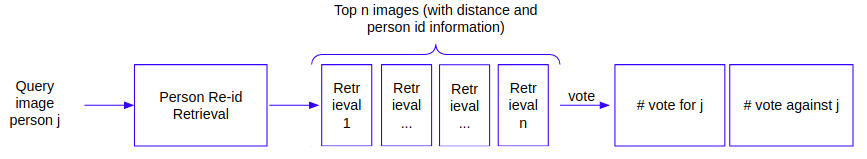
\includegraphics[width=\textwidth]{figures/second_idea.png}

Now, if the person re-id system is specified as in figure above, we can calculate $P(\overrightarrow{v} \mid query = j)$ with $\overrightarrow{v} = <\#vote\_for, ~\#vote\_againts>$ by iterating each image of each person on the training set. Using this probability we know how likely that the voting goes right (or wrong) given a query of person $j$. Using this probability we can work out, using Bayesian inference, $P(query=j \mid \overrightarrow{v})$ as:

\begin{equation}
	\label{eq:second_idea}
	\begin{tabular}{r@{=}l}
		$P(query=j \mid \overrightarrow{v})$ & $\frac{\displaystyle P(\overrightarrow{v} \mid query = j) P(query=j)}{\displaystyle\sum_{k=1}^{K} P(\overrightarrow{v} \mid query = k) P(query=k)}$ \\ 
	\end{tabular}
\end{equation}

\noindent with $K$ the total persons.
\\
\\
\noindent \textbf{Problems:}
This idea is a bit odd, it can be seen from equation \ref{eq:second_idea}, because given the configuration voting $<v_f, v_a>$, then we want to know how likely the query person $j$ is. The $P(\overrightarrow{v} \mid query = j)$ seems more like a proportion of voting configuration for each person $j$.

If we just calculate $P(<v_f, v_a>)$, then this just tells us the proportion of the voting configuration based on the training data.

How can we transform this into, perhaps, a ratio of $\displaystyle\frac{P_j}{\Sigma_{i \neq j} P_i}$? 

\section{Third Idea}

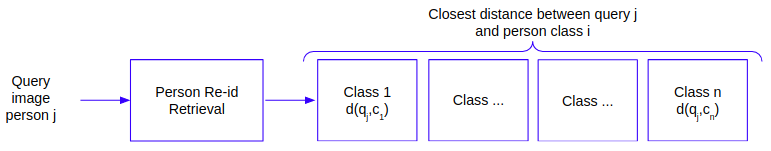
\includegraphics[width=\textwidth]{figures/third_idea.png}

Using the specified re-id system as in figure above with $d(q_j, c_i)$ as the closest distance value between the query of person $j$ and the person classification $c_i$ (the person is classified as $i$), we can calculate the probability $P(d(q_j, c_i) \mid c_i)$ using the (general) distributions over the distance for both matched image and negative images (graphs shown in Figure \ref{fig:match_mismatch_dist}). Using this probability we can work out, using Bayesian inference, $P(c_i \mid d(q_j, c_i))$ as:

\begin{equation}
	\label{eq:third_idea}
	\begin{tabular}{r@{=}l}
		$P(c_i \mid d(q_j, c_i))$ & $\frac{\displaystyle P(d(q_j, c_i) \mid c_i) P(c_i)}{\displaystyle\sum_{k=1}^{n} P(d(q_j, c_k) \mid c_k) P(c_k)}$ \\ 
	\end{tabular}
\end{equation}

\noindent with $n$ the total persons. However, this only works out if the person retrieval system provides the distance $d(q_j, c_i)$ for all $1 \leq i \leq n$ in each query.

\begin{figure*}
	\centering
	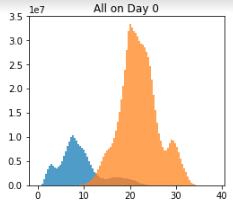
\includegraphics[width=0.40\textwidth]{./figures/match_mismatch_dist.png}
	\caption{Assuming this is a distribution over distance with blue is a distribution for matched query-image ($q_j = c_i$) and orange is a distribution for negative images ($q_j \neq c_i$).}
	\label{fig:match_mismatch_dist}
\end{figure*}

Given particular time interval $m$ where a series of $m$ query images of person $j$ is fed to the system producing distances $d(q_{1j}, c_{1i}), \ldots, d(q_{mj}, c_{mi})$, then the probability $P(\overrightarrow{c_i} \mid \overrightarrow{d(q_j, c_i)})$ can be defined as:

\begin{equation}
	\label{eq:joint_third_idea}
	\begin{tabular}{r@{=}l}
		$P(\overrightarrow{c_i} \mid \overrightarrow{d(q_j, c_i)})$ & $\displaystyle \prod_{k=1}^{m} P(c_{ki} \mid d(q_{kj}, c_{ki}))$ \\ 
	\end{tabular}
\end{equation}

\noindent with $\overrightarrow{c_i} = (c_{1i}, \ldots, c_{mi})$, and $\overrightarrow{d(q_j, c_i)} = (d(q_{1j}, c_{1i}), \ldots, d(q_{mj}, c_{mi}))$.

\end{document}